\section{Details}
This section describes the details necessary for the implementation of the different modules.

\begin{figure}
\begin{center}
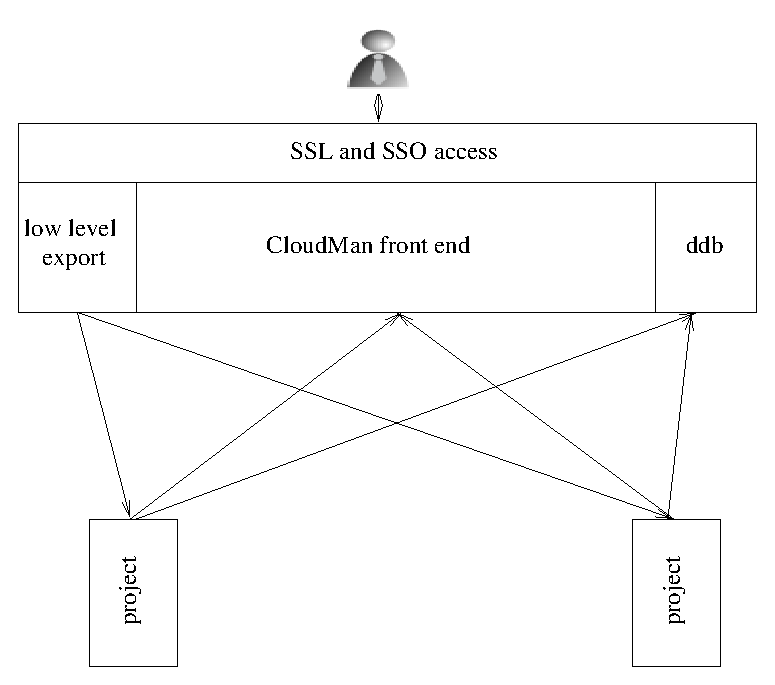
\includegraphics[width=0.9\textwidth]{cloudman_highlevel.eps}
\caption{\label{architecture} Updated architecture of the desired system. Users connect to the front-end which offers a graphical user interface. The side is secured with SSL techniques. All users have to authenticate using the sites Single Sign On mechanism. The data which is entered is stored in an external database and exported in a low level format. Shown in this figure are project specific backends only. In general these backends are site specific, and design to configure specific services. Each backend reads the data which it needs to configure it's resources from the low level export layer from CloudMan. The current state which includes error or warning conditions is reported back to the frontend as well as the CloudMan database. The database is used to record the historical state data per project backend.}
\end{center}
\end{figure}
Fig.~\ref{architecture} shows an overview over the CloudMan architecture. Users have to authenticate using SSO. After login, the communication stays secured by SSL. Project backends report their state asynchronously via a file or URL. The state data is recorded in the database to save the history. 
